\documentclass{article}
\begin{document}
\subsection{Running example on MCU side via BLE}
The sequence of actions required for interfacing via BLE includes the steps below:
\begin{enumerate}
	\item Go to the \path{examples} folder in file explorer
	\item Open the common.c file in the selected example folder in your IDE
	\item Change COINES\_COMM\_INTF\_USB  to COINES\_COMM\_INTF\_BLE
	\begin{figure}[H]
		\begin{center}
			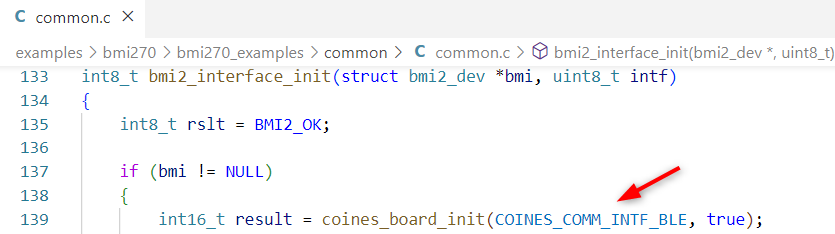
\includegraphics[width=0.9\textwidth]{coinesAPI_images/Mcu_example_ble_intf.png}
		\end{center}
	\end{figure}
	\item Open example script and change the 
	\begin{verbatim}
	printf(...) to fprintf(bt_w,...)
	\end{verbatim}
	\begin{figure}[H]
		\begin{center}
			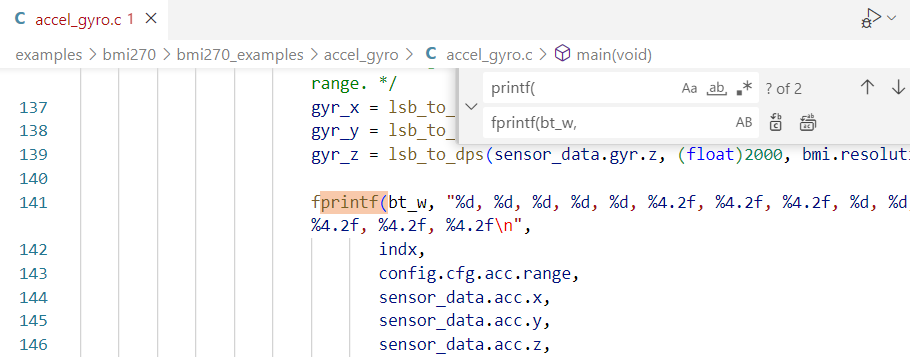
\includegraphics[width=0.9\textwidth]{coinesAPI_images/Mcu_example_ble_print.png}
		\end{center}
	\end{figure}
	\item Now follow the same steps from 1 - 4 in the above section.
	\item Connect the Application board to another power source and keep it within the BLE range.
	\item View the output in the \href{https://wiki.makerdiary.com/web-device-cli/}{Web Device CLI} site in your browser by connecting to board via BLE.
	\begin{figure}[H]
		\begin{center}
			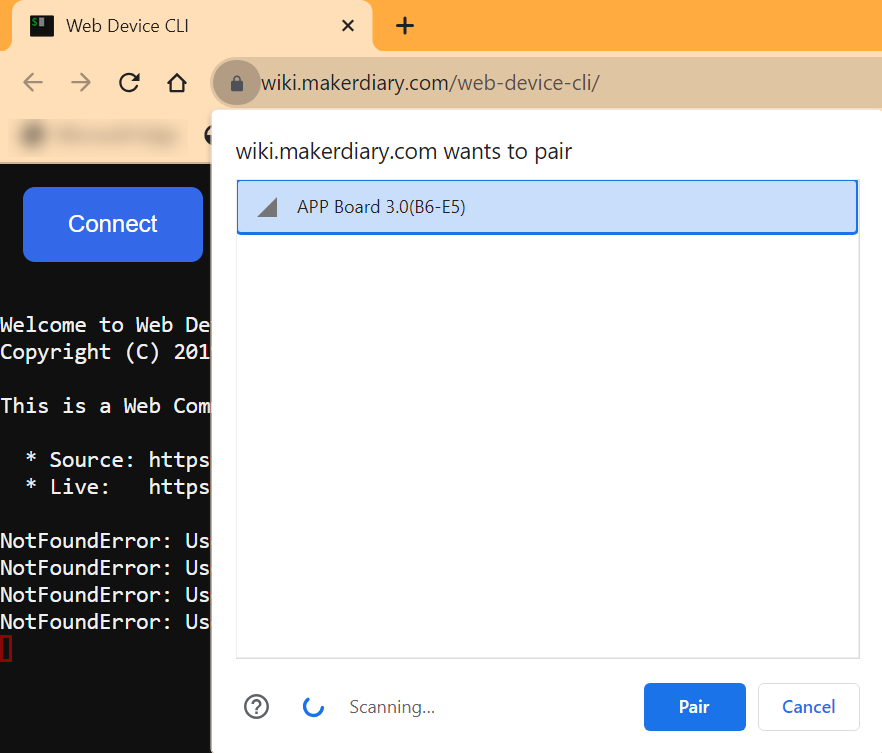
\includegraphics[width=0.7\textwidth]{coinesAPI_images/Mcu_example_ble_pair.png}
		\end{center}
	\end{figure}
	\begin{figure}[H]
		\begin{center}
			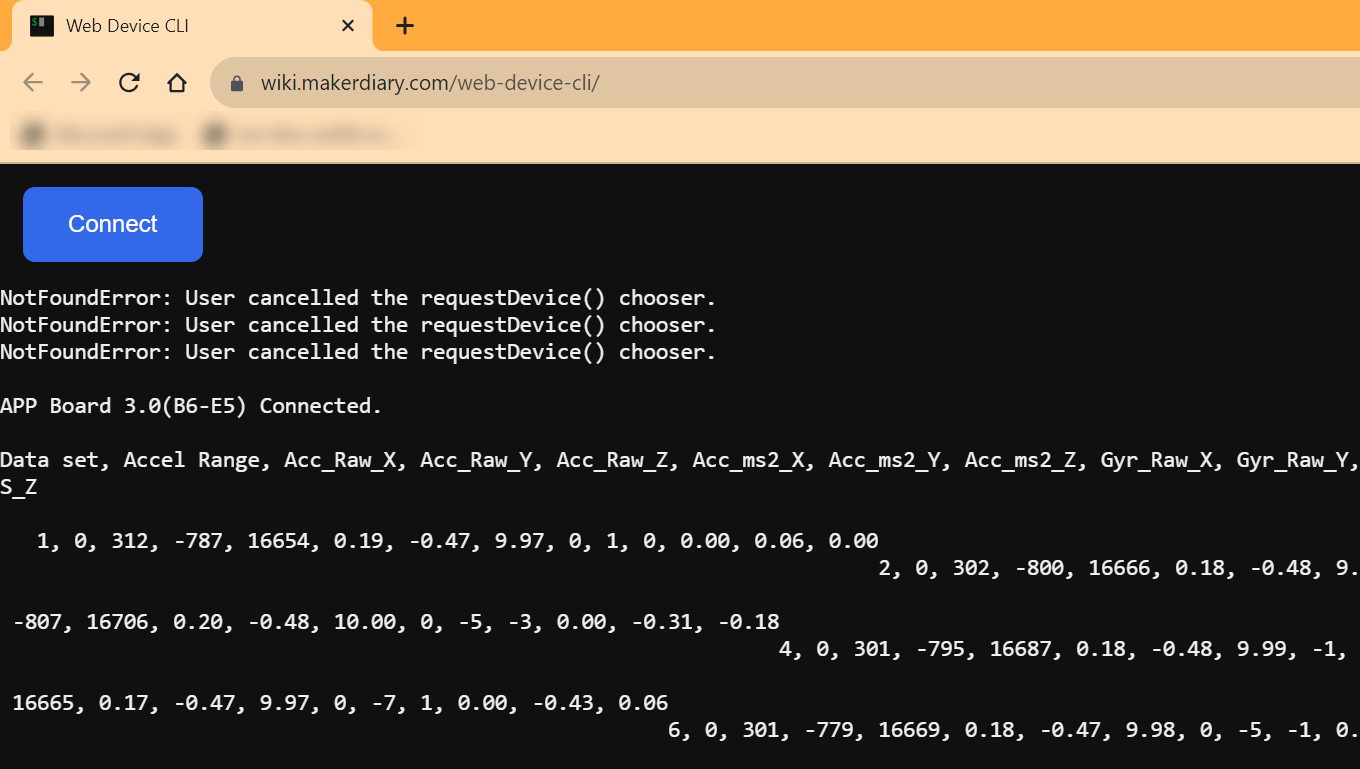
\includegraphics[width=0.9\textwidth]{coinesAPI_images/Mcu_example_ble_output.png}
		\end{center}
	\end{figure}
\end{enumerate}



\end{document}